\chapter{Background}

\section{Theoretical Background}

To establish the mathematics basis and mental model of the problem, some essential conceptions in Computer Graphics are going to be introduced in this chapter.  

\subsection{Radiometry Introduction}
Radiometry is the basic terminology to describe light which is crucial to simulation. First of all, some basic quantities have to be introduced, the related symbols are going to be defined here as well for further use.

\paragraph{Important Quantities} 

\begin{table}[!ht]
\begin{center}
	\begin{tabular}{ | l | l | l |}     	
	\hline 

	Symbol & Quantity & Unit \\

	% \(Q_{\lambda}\) 	& 		Spectral radiant energy 		& 		\(J nm^{-1} \) \\
	\(Q\) 			& 		Radiant Energy 				& 		\(j\) \\ 
	\(\Phi\) 			& 		Radiant flux 					& 		\(W\) \\ 
	\(I\) 			& 		Radiant intensity 				& 		\(W sr^{-1}\) \\
	\(E\)			&		Irradiance (incident) 			&		\(W m^{-2}\) \\  
	\(L\)			&		Radiance						&		\(W m^{-2} sr^{-1}\) \\ 
	
	\hline

	\end{tabular}
\end{center} 
\caption{Radiometric symbols, names and units.}
\label{tab:radiometry_quantities}
\end{table}

\emph{Radiant energy}, \(Q\), is the energy of a collection of photons which is the basic quantity in lighting. 

\emph{Radiant flux} , \(\Phi\), is the time rate of the flow of radiant energy passing through a surface or region of space. Total emission from a light source is generally described in terms of flux. \ref{fig:flux_point_light} shows the flux emitted from a point light source measured by the total amount of energy passing through an virtual sphere around the light. 

\begin{figure}[htp] 
    \centering 
    \fbox{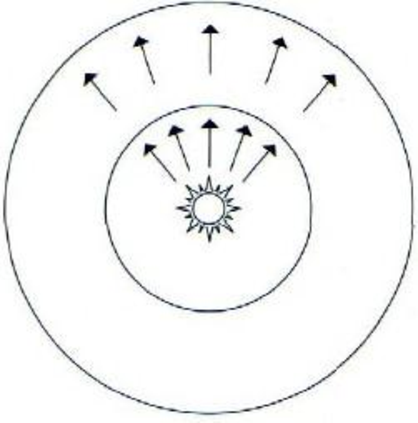
\includegraphics{flux.pdf}}
    \renewcommand{\thefigure}{\thechapter.\arabic{figure}}
    \caption[]{Radiant flux from a point light source is passing through the spheres around the light.}
    \label{fig:flux_point_light} 
\end{figure} 

\emph{Irradiance}, \(E\), is the incident (arriving at a surface location) \emph{radiant flux area density}, which is defined as the differential flux per differential area. While \emph{Radiant exitance} denoted by \(M\) is area density of flux leaving a surface.  

\begin{equation}
E(x) = \frac{d\Phi}{dA}
\end{equation}

\emph{Radiance}, \(L\), is the radiant flux per unit solid angle per unit projected area: 

\begin{equation}
L(x, \overrightarrow{\omega}) = \frac{d^{2}\Phi}{\cos{\theta} \cdot dA \cdot d\overrightarrow{\omega}}
\end{equation}

Where \(x\) is the position and \(\overrightarrow{\omega}\) is the direction. 

Radiance is the most important quantity in rendering simulation since it closely represent the color. Also radiance can be considered as the number of photons arriving per time at a small area from a given direction. Radiant energy can be computed by integrating the radiance field over all directions \(\Omega\) and area \(A\).

\begin{equation} 
\Phi = \int_{A}\int_{\Omega}L(x, \overrightarrow{\omega})(\overrightarrow{\omega} \cdot \overrightarrow{n})d\overrightarrow{\omega}dx
\label{eq:flux_from_radiance}
\end{equation} 

\begin{figure}[htp] 
    \centering 
    \fbox{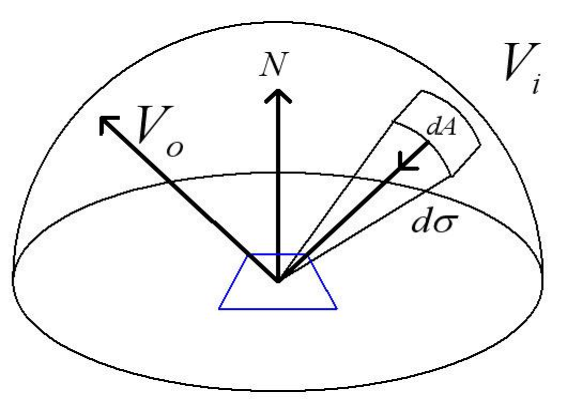
\includegraphics{solid_angle_sphere.pdf}}
    \renewcommand{\thefigure}{\thechapter.\arabic{figure}}
    \caption[]{Radiance, L, is defined as the radiant flux per unit solid angle, \(\overrightarrow{\omega}\), per unit projected area, \(dA\)}
    \label{fig:solid_angle_sphere} 
\end{figure}

The solid angle used in equation \ref{eq:flux_from_radiance} can be thought as representation of both a direction and an infinitesimal area. Therefore solid angle can also be expressed in spherical coordinates (\(\theta, \phi\))

\begin{figure}[htp] 
    \centering 
    \fbox{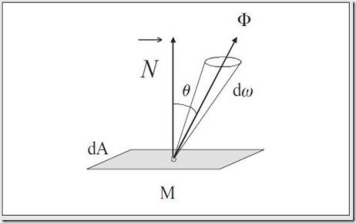
\includegraphics[width=\linewidth]{radiance_solid_angle.pdf}}
    \renewcommand{\thefigure}{\thechapter.\arabic{figure}}
    \caption[]{Radiance, L, is defined as the radiant flux per unit solid angle, \(\overrightarrow{\omega}\), per unit projected area, \(dA\)}
    \label{fig:radiance_solid_angle} 
\end{figure} 

\paragraph{Light Emission}

\paragraph{}








